%%%%%%%%%%%%%%%%%%%%%%%%%%%%%%%%%%%%%%%%%
% Simple Sectioned Essay Template
% LaTeX Template
%
% This template has been downloaded from:
% http://www.latextemplates.com
%
% Note:
% The \lipsum[#] commands throughout this template generate dummy text
% to fill the template out. These commands should all be removed when 
% writing essay content.
%
%%%%%%%%%%%%%%%%%%%%%%%%%%%%%%%%%%%%%%%%%

%----------------------------------------------------------------------------------------
%	PACKAGES AND OTHER DOCUMENT CONFIGURATIONS
%----------------------------------------------------------------------------------------

\documentclass[12pt]{article} % Default font size is 12pt, it can be changed here

\usepackage{geometry} % Required to change the page size to A4
\geometry{a4paper} % Set the page size to be A4 as opposed to the default US Letter

\usepackage{graphicx} % Required for including pictures

\usepackage{float} % Allows putting an [H] in \begin{figure} to specify the exact location of the figure


\usepackage{lipsum} % Used for inserting dummy 'Lorem ipsum' text into the template

\linespread{1.2} % Line spacing

%\setlength\parindent{0pt} % Uncomment to remove all indentation from paragraphs

\graphicspath{{Pictures/}} % Specifies the directory where pictures are stored

\begin{document}

%----------------------------------------------------------------------------------------
%	TITLE PAGE
%----------------------------------------------------------------------------------------

\begin{titlepage}

\newcommand{\HRule}{\rule{\linewidth}{0.5mm}} % Defines a new command for the horizontal lines, change thickness here

\center % Center everything on the page

\textsc{\LARGE Politecnico di Milano}\\[1.5cm] % Name of your university/college
\textsc{\Large Dipartimento di elettronica, informazione e bioingegneria}\\[0.5cm] % Major heading such as course name
\textsc{\large Image analysis}\\[0.5cm] % Minor heading such as course title

\HRule \\[0.4cm]
{ \huge \textbf{ Software for traffic violation of 
\\ a right hand rule}}\\[0.4cm] % Title of your document
\HRule \\[1.5cm]

\begin{minipage}{0.4\textwidth}
\begin{flushleft} \large
\emph{Author:}\\
Mirjam \textsc{Skarica},\\ 
Lucija \textsc{Megla} % Your name
\end{flushleft}
\end{minipage}
~
\begin{minipage}{0.4\textwidth}
\begin{flushright} \large
\emph{Supervisor:} \\
prof. Vincenzo \textsc{Caglioti} % Supervisor's Name
\end{flushright}
\end{minipage}\\[4cm]

{\large \today}\\[3cm] % Date, change the \today to a set date if you want to be precise

%\includegraphics{Logo}\\[1cm] % Include a department/university logo - this will require the graphicx package

\vfill % Fill the rest of the page with whitespace

\end{titlepage}

%----------------------------------------------------------------------------------------
%	TABLE OF CONTENTS
%----------------------------------------------------------------------------------------

\tableofcontents % Include a table of contents

\newpage % Begins the essay on a new page instead of on the same page as the table of contents 

%----------------------------------------------------------------------------------------
%	INTRODUCTION
%----------------------------------------------------------------------------------------

\section{Introduction} % Major section

In the last few decades there has been a huge growth of traffic in the big cities. In consequence with growth of traffic, number of violations increased. As a result, software for traffic violation detection is a way to maintain order and track violations in a profitable way.

%------------------------------------------------

\subsection{Motivation and formulation of the problem} % Sub-section

Even though many crossroads have traffic lights or traffic signs, there are still crossroads without any of it. As many know, in that particular case right-hand rule is applied. In absence of traffic lights or signs, right hand rule demands from a driver of a vehicle to give away the priority to vehicles approaching from the right at intersections.

Given the above problem, the goal of the project is to develop a software that is going to recognize violations of the right hand rule and inform the operator about it. This way, we could gain an automated way to recognize this type of violations, which could help track situations on every intersection without traffic lights or signs. This is going to make tracking of right hand rule violations far more easier and profitable.

%------------------------------------------------

\subsection{Camera and acquisition of video material} % Sub-section

Formulation of the project for developing software for right-hand rule violations guarantees acquisition of the video material through a traffic surveillance camera placed in an elevated area. 
Since we did not have a surveillance camera at our disposal, we used a classical digital camera attached to an elevated object. Our camera had a frame rate of 30 fps and was attached to a trivet to reduce vibrations and other disturbances in order to capture a credible situation.



%------------------------------------------------

\subsection{Document structure}

This document serves to describe the structure of the software and its implementation in detail. Also, a detailed utility manual is given to describe software use-cases and to give a glimpse of situations in which software will work and some situations in which might fail.
\\

The report is divided into three sections:
\begin{enumerate}
\item Structure of the software and its implementation, in which we describe in detail approached used in development of our software;
\item Manual, in which we describe possible use cases of the software;
\item Conclusion, in which we give a critical review of our software and we list possible improvements of it. 
\end{enumerate}

%------------------------------------------------


%----------------------------------------------------------------------------------------
%	MAJOR SECTION 1
%----------------------------------------------------------------------------------------

\section{Structure of the software and its implementation} % Major section

To get a software that recognizes traffic violations of a right hand rule, we had to divide the task in more subtasks to get the desired behaviour. Those subtasks can be seen in Figure 1.

\begin{figure}[ht]
\centering
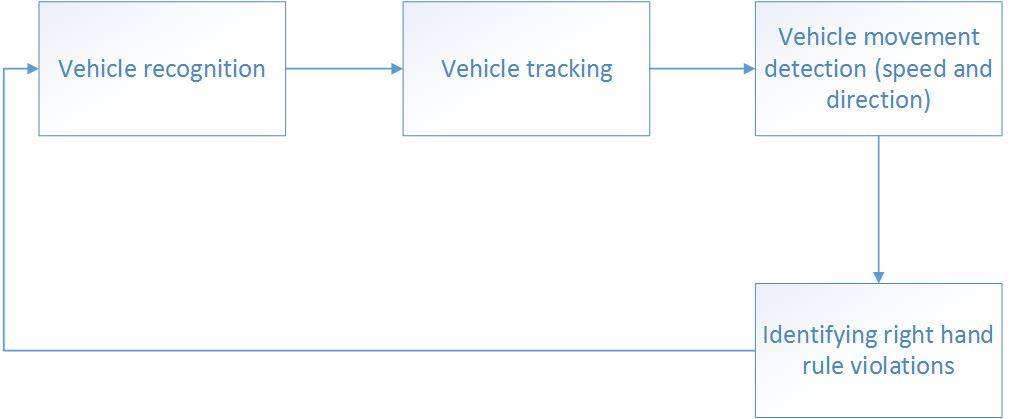
\includegraphics[width=10cm]{Drawing1.jpg}
\caption{Software work flow}
\end{figure}

As we can see from Figure 1., first step in our algorithm consist of car recognition. In this step we had to extract background from the foreground and recognize cars in the given foreground. After extracting vehicles from the video footage, we had to track them through frames, so that we could determine their speed and direction. To identify if there is a violation of the right hand rule in the intersection, we divided the intersection in priorities and with the help of car's direction and speed determined if the violation occurred or not.

%------------------------------------------------

\subsection{Vehicle recognition} % Sub-section

When we look at problems video surveillance could solve, we need to make sure the system is robust. To say the system of video surveillance is robust, it should not depend on correct position of the camera and it should not lose its performance when there are:

\begin{enumerate}
\item[•] objects that can be partially seen in the scene
\item[•] overlapping objects in the scene
\item[•] shadows
\item[•] changes of lightning
\item[•] objects that move slowly
\item[•] objects that were visible and then removed from the scene

\end{enumerate}

Talking about recognizing of vehicles, the problem of their identification consists mostly of being able to keep good estimation of the foreground. After that, applying filters to foreground estimation will give us a foreground with more quality in which we can extract vehicles with \textit{blob analysis}.
In the next few paragraphs we are going to explain all three steps in detail.

\subsubsection{Foreground estimation}

Major part of foreground estimation approaches are based on background estimation, which do not apply on our problem, that is, they did not give good results. That is why we chose to work with Gaussian Mixture Models (GMM), which gave us flexibility and robustness to confront all the problems stated above. Although different methods of GMM exist, like the one of Friedman and Russell ([FR97]), which explicitly classifies values of pixels with three different distributions and determines if the pixels belong to the street, shadows or vehicles, the method implemented in our software is the one of Stauffer and Grimson [SG99]. This method of GMM does not model all the pixels with one particular distribution, but models the value of one pixel with mixture of different Gaussians; the motive for using mixture of different Gaussians lies in the fact that  multiple surfaces often appear in the view frustum of a particular pixel and the lighting conditions change. Hence, mixture of Gaussians is able to surpass those changes. Each time the parameters of the Gaussians are updated,
the Gaussians are evaluated using a simple
heuristic to hypothesize which are most likely to be part of the "background process". Pixel values that do not match one of the pixel’s "background" Gaussians are grouped using connected components. Finally, the connected components are tracked from frame to frame using a multiple hypothesis tracker. 
This method uses two parameters: $\alpha$ and $T$. Parameter $\alpha$ represents learning rate and parameter $T$ is a threshold for determining which distributions belong to the background and which do not.  

We consider the values of a particular pixel over
time as a "pixel process". The "pixel process" is a
time series of pixel values, e.g. scalars for gray values or vectors for color images. At any time $t$, what is known about a particular pixel, ${x_{0}, y_{0}}$, is its history:

\begin{equation}
{\{X_{1},X_{2},...,X_{t}} = {I(x_{0},y_{0},i):1\leq i \leq t\}}
\end{equation}

where $I$ is the image sequence. The recent history of each pixel, ${X_{1}, ..., X_{t}}$, is modeled by a mixture of K Gaussian distributions. The probability of observing the current pixel value is

\begin{equation}
{P(X_{t}) = \sum_{i=1}^{K}\omega_{i,k} \ast \eta(X_{t},\mu_{i,t}, \sum_{i,t})}
\end{equation}

where $K$ is the number of distributions, $\omega_{i,t}$ is an estimate
of the weight (what portion of the data is accounted for by this Gaussian) of the $i$-th Gaussian in the mixture at time $t$, $\mu_{i,t}$ is the mean value of the $i$- th Gaussian in the mixture at time $t$, $\sum_{i,t}$ is the covariance matrix of the $i$-th Gaussian in the mixture at time $t$, and where $\eta$ is a Gaussian probability density function:

\begin{equation}
\eta(X_{t},\mu_{i,t}, \sum_{i,t} = \frac{1}{(2\pi)^{\frac{n}{2}}|\sum|^{\frac{1}{2}}} e^{-\frac{1}{2}(X_{t}-\mu_{t})^{T}\sum^{-1}(X_{t}-\mu_{t})}
\end{equation}

K can take values between 3 and 5. In this case, 5 is used. Also, for computational reasons, the covariance matrix is assumed to be of the form:

\begin{equation}
{\sum_{k,t} = \sigma_{k}^{2}\textbf{I}}
\end{equation}

This assumes that the red, green, and blue pixel values are independent and have the same variances. While this is certainly not the case, the assumption allows us to avoid a costly matrix inversion at the expense of some accuracy. 
Thus, the distribution of recently observed values
of each pixel in the scene is characterized by a mixture of Gaussians. A new pixel value will, in general, be represented by one of the major components of the mixture model and used to update the model. 

%------------------------------------------------





%----------------------------------------------------------------------------------------
%	MAJOR SECTION X - TEMPLATE - UNCOMMENT AND FILL IN
%----------------------------------------------------------------------------------------

%\section{Content Section}

%\subsection{Subsection 1} % Sub-section

% Content

%------------------------------------------------

%\subsection{Subsection 2} % Sub-section

% Content

%----------------------------------------------------------------------------------------
%	CONCLUSION
%----------------------------------------------------------------------------------------

\section{Conclusion} % Major section


%----------------------------------------------------------------------------------------
%	BIBLIOGRAPHY
%----------------------------------------------------------------------------------------

\begin{thebibliography}{99} % Bibliography - this is intentionally simple in this template

\bibitem[Figueredo and Wolf, 2009]{Figueredo:2009dg}
Figueredo, A.~J. and Wolf, P. S.~A. (2009).
\newblock Assortative pairing and life history strategy - a cross-cultural
  study.
\newblock {\em Human Nature}, 20:317--330.
 
\end{thebibliography}

%----------------------------------------------------------------------------------------

\end{document}